\subsection{Аддитивные свойства интеграла Римана}

В данном билете рассматривается свойство аддитивности интеграла как функции отрезка. Лектор отмечает, что это свойство имеет прозрачную физическую интерпретацию: если рассматривать интеграл как перемещение точки при заданной скорости, то общее перемещение за весь промежуток времени равно сумме перемещений за его отдельные части.

\subsubsection*{1. Интегрируемость на части отрезка}

\begin{theorem}
Пусть функция $f(x)$ интегрируема по Риману на отрезке $[a, b]$. Если отрезок $[c, d]$ содержится в $[a, b]$ ($[c, d] \subset [a, b]$), то функция $f(x)$ также интегрируема на отрезке $[c, d]$.
\end{theorem}

\begin{tcolorbox}[title=Доказательство, breakable]
Для доказательства воспользуемся критерием Дарбу: функция интегрируема тогда и только тогда, когда для любого $\eps > 0$ существует разбиение, разность сумм Дарбу для которого меньше $\eps$.

1. Так как $f \in R([a, b])$, то по критерию Дарбу для любого $\eps > 0$ существует такое $\delta > 0$, что для любого разбиения $P$ отрезка $[a, b]$ с диаметром $\lambda(P) < \delta$ выполняется:
\[ \sum_{j=1}^n \omega_j \Delta x_j < \eps \]
где $\omega_j$ — колебание функции на элементарном отрезке.

2. Рассмотрим произвольное разбиение $\pi$ отрезка $[c, d]$ с диаметром $\lambda(\pi) < \delta$. Дополним это разбиение точками на множестве $[a, b] \setminus [c, d]$ так, чтобы получить разбиение $P$ всего отрезка $[a, b]$ с диаметром $\lambda(P) < \delta$.

3. Сумма колебаний для разбиения $P$ состоит из неотрицательных слагаемых. Слагаемые, соответствующие разбиению $\pi$ отрезка $[c, d]$, являются частью этой суммы:
\[ \sum_{\pi} \omega_k \Delta x_k \le \sum_{P} \omega_j \Delta x_j < \eps \]

4. Таким образом, для любого $\eps > 0$ мы нашли $\delta$, такое что любое разбиение отрезка $[c, d]$ мелкости меньше $\delta$ удовлетворяет критерию Дарбу. Следовательно, функция интегрируема на $[c, d]$.
\end{tcolorbox}

\subsubsection*{2. Основная теорема об аддитивности}

\begin{theorem}
Пусть $a < c < b$. Функция $f(x)$ интегрируема на отрезке $[a, b]$ тогда и только тогда, когда она интегрируема на обоих отрезках $[a, c]$ и $[c, b]$. При этом справедливо равенство:
\[ \int_a^b f(x) dx = \int_a^c f(x) dx + \int_c^b f(x) dx \]
\end{theorem}

\begin{tcolorbox}[title=Доказательство, breakable]
Доказательство состоит из двух частей: обоснование интегрируемости и вывод формулы.

\textbf{1. Интегрируемость.} 
Необходимость (если интегрируема на $[a, b]$, то на $[a, c]$ и $[c, b]$) доказана в предыдущей теореме.
Докажем достаточность. Пусть $f$ интегрируема на $[a, c]$ и $[c, b]$. Тогда она ограничена на каждом из них, а значит, ограничена числом $M$ на всем $[a, b]$. 
Для любого $\eps > 0$ существуют $\delta_1$ и $\delta_2$, такие что суммы колебаний на $[a, c]$ и $[c, b]$ меньше $\eps$. Возьмем $\delta = \min(\delta_1, \delta_2, \eps/M)$. 
При произвольном разбиении $P$ отрезка $[a, b]$ мелкости $\lambda(P) < \delta$ разделим его сумму колебаний на три части:
\begin{itemize}
    \item $\sum'$ — по отрезкам, лежащим целиком внутри $[a, c]$. Она меньше $\eps$.
    \item $\sum''$ — по отрезкам, лежащим целиком внутри $[c, b]$. Она также меньше $\eps$.
    \item $\sum_{c}$ — по отрезкам (их не более двух), содержащим точку $c$. Колебание на них $\le 2M$, а суммарная длина $\le 2\delta$. Тогда эта часть $\le 4M\delta < 4\eps$.
\end{itemize}
Итоговая сумма колебаний на $[a, b]$ меньше $6\eps$, что доказывает интегрируемость.

\textbf{2. Равенство.}
Возьмем произвольное разбиение $P$ отрезка $[a, b]$, в которое \textbf{обязательно включим} точку $c$ как точку разбиения. Тогда любая интегральная сумма Римана для $f(x)$ на $[a, b]$ распадается на две суммы:
\[ \sigma(f, P, \xi) = \sum_{[a, c]} f(\xi_k) \Delta x_k + \sum_{[c, b]} f(\xi_j) \Delta x_j \]
При $\lambda(P) \to 0$ левая часть по определению стремится к $\int_a^b f(x) dx$. Правые слагаемые стремятся к интегралам по $[a, c]$ и $[c, b]$ соответственно. В силу единственности предела получаем искомое равенство.
\end{tcolorbox}

\subsubsection*{3. Обобщение на случай произвольного расположения точек}

Лектор вводит расширенное определение интеграла, позволяющее отказаться от условия $a < b$:
\begin{enumerate}
    \item Если $a > b$, то $\int_a^b f(x) dx = -\int_b^a f(x) dx$.
    \item Если $a = b$, то $\int_a^a f(x) dx = 0$.
\end{enumerate}

С учетом этого определения аддитивность формулируется максимально широко:

\begin{theorem}
Пусть $f(x)$ интегрируема на наибольшем из отрезков, концами которых являются точки $a, b, c \in \R$. Тогда:
\[ \int_a^b f(x) dx + \int_b^c f(x) dx + \int_c^a f(x) dx = 0 \]
Или, что эквивалентно:
\[ \int_a^c f(x) dx = \int_a^b f(x) dx + \int_b^c f(x) dx \]
\end{theorem}

\begin{tcolorbox}[title=Доказательство, breakable]
Рассмотрим случай, когда $\max(a, b, c) = c$ и $\min(a, b, c) = a$. Тогда по доказанному выше для $a \le b \le c$:
\[ \int_a^c f(x) dx = \int_a^b f(x) dx + \int_b^c f(x) dx \]
Перенесем интеграл по $[a, c]$ в правую часть со знаком минус:
\[ 0 = \int_a^b f(x) dx + \int_b^c f(x) dx - \int_a^c f(x) dx \]
Используя определение $\int_c^a = -\int_a^c$, получаем:
\[ \int_a^b f(x) dx + \int_b^c f(x) dx + \int_c^a f(x) dx = 0 \]
Любые другие варианты расположения точек $a, b, c$ доказываются аналогичной перестановкой пределов интегрирования.
\end{tcolorbox}

\subsubsection*{Геометрический смысл}
Геометрически аддитивность означает, что площадь фигуры, ограниченной графиком на отрезке $[a, b]$, складывается из площадей её частей над подотрезками. В физическом смысле (работа силы или путь) это означает независимость результата от того, вычисляется ли он за один этап или как сумма результатов на последовательных участках пути. При этом учет направления движения (знак интеграла) позволяет рассматривать точки в любом порядке.

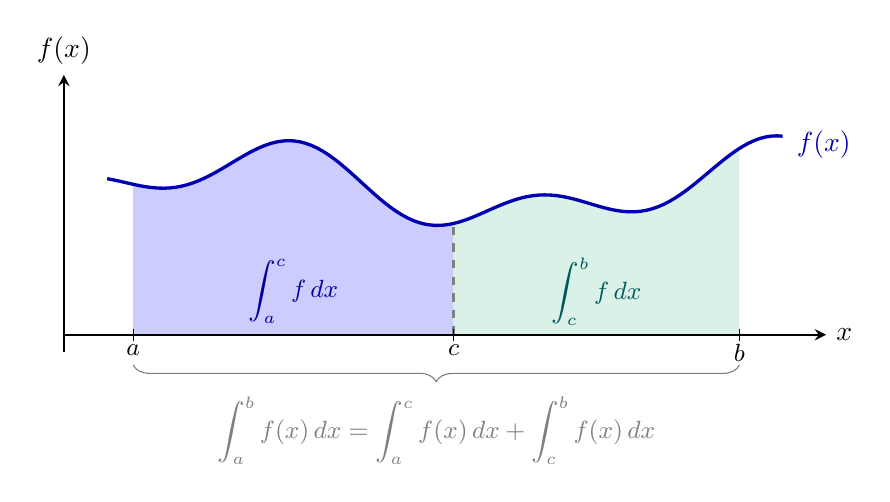
\begin{tikzpicture}[>=stealth, scale=1.1]
 
% ИСПРАВЛЕНО: используем #1 вместо \x внутри \pgfmathdeclarefunction
\pgfmathdeclarefunction{ff}{1}{%
  \pgfmathparse{0.35*sin(deg(#1-0.5))+1.7+0.25*cos(deg(2.3*#1))}%
}
 
\def\xa{0.8}
\def\xc{4.5}
\def\xb{7.8}
 
%--- Область от a до c (синяя) ---
\fill[blue!20,domain=\xa:\xc,samples=80]
  plot(\x,{ff(\x)}) -- (\xc,0) -- (\xa,0) -- cycle;
 
%--- Область от c до b (зелёная) ---
\fill[green!25!teal!15,domain=\xc:\xb,samples=80]
  plot(\x,{ff(\x)}) -- (\xb,0) -- (\xc,0) -- cycle;
 
%--- Кривая ---
\draw[blue!70!black, very thick, domain=0.5:8.3, samples=120]
  plot(\x,{ff(\x)});
 
%--- Вертикальная линия в c ---
\pgfmathsetmacro{\fc}{ff(\xc)}
\draw[gray,dashed,thick] (\xc,0)--(\xc,\fc);
 
%--- Оси ---
\draw[->,thick] (0,0)--(8.8,0) node[right]{$x$};
\draw[->,thick] (0,-0.2)--(0,3.0) node[above]{$f(x)$};
 
%--- Метки a, c, b ---
\foreach \xp/\lab in {\xa/{$a$},\xc/{$c$},\xb/{$b$}}{
  \draw (\xp,0.07)--(\xp,-0.07);
  \node[below,font=\small] at (\xp,0) {\lab};
}
 
%--- Надписи на областях ---
\node[blue!60!black,font=\small] at ({(\xa+\xc)/2},0.5)
  {$\displaystyle\int_a^c f\,dx$};
\node[teal!70!black,font=\small] at ({(\xc+\xb)/2},0.5)
  {$\displaystyle\int_c^b f\,dx$};
 
%--- Фигурная скобка снизу ---
\draw[decorate,decoration={brace,amplitude=6pt,mirror},gray]
  (\xa,-0.35)--(\xb,-0.35)
  node[midway,below=8pt,font=\small]
    {$\displaystyle\int_a^b f(x)\,dx
      = \int_a^c f(x)\,dx + \int_c^b f(x)\,dx$};
 
\node[blue!70!black,font=\itshape,right] at (8.35,2.2){$f(x)$};
 
\end{tikzpicture}
